\documentclass[UTF8]{ctexart}
\usepackage{geometry}
\usepackage{listings}
\usepackage{xcolor}
\usepackage{graphicx}
\usepackage{float}
\usepackage{multirow}
\usepackage{array}
\usepackage{longtable}
\usepackage{hyperref}
\usepackage{ctex}

\geometry{a4paper,scale=0.8}
\lstset{
    numbers=left, %设置行号位置
    numberstyle=\tiny, %设置行号大小
    keywordstyle=\color{blue}, %设置关键字颜色
    commentstyle=\color[cmyk]{1,0,1,0}, %设置注释颜色
    frame=single, %设置边框格式
    escapeinside=``, %逃逸字符(1左面的键),用于显示中文
    breaklines, %自动折行
    extendedchars=false, %解决代码跨页时,章节标题,页眉等汉字不显示的问题
    xleftmargin=2em,xrightmargin=2em, aboveskip=1em, %设置边距
    tabsize=4, %设置tab空格数
    showspaces=false %不显示空格
    }
\hypersetup{
    colorlinks=true,
    linkcolor=black,
    citecolor=black
}
\title{计算机系统结构实验报告\\实验3}

\date{\today}
\begin{document}
\maketitle
\begin{abstract}
    本实验实现了简单的类MIPS处理器的几个重要部件:主控制器(Ctr)、运算单元控制器(ALUCtr)以及算术逻辑运算单元(ALU),其作用分别是产生处理器所需要的各种控制信号、产生算术逻辑运算单元(ALU)所需要的控制信号以及根据运算单元控制器(ALUCtr)发出的信号执行相应的算术逻辑运算输出结果。本实验通过软件仿真的形式进行实验结果的验证。
\end{abstract}
\tableofcontents
\clearpage
\section{实验目的}
\begin{enumerate}
    \item 理解CPU控制器、ALU的原理
    \item 主控制器(Ctr)的实现
    \item 运算单元控制器(ALUCtr)的实现
    \item ALU的实现
    \item 功能仿真
\end{enumerate}
\section{原理分析}\label{sec1}
\subsection{主控制器模块}
主控制器(Ctr)的输入为指令的操作码(opCode)字段,主控制器模块对操作码进行译码,向ALU控制器、寄存器、数据选择器等部件输出正确的控制信号。\par
本实验中,主控制器模块可以识别R型指令、lw、sw、beq、jump指令并输出对应的控制信号。控制器产生的控制信号如表\ref{tab:ctr-sig-name}所示。
\begin{table}[htbp]
    \centering
    \resizebox{\textwidth}{!}{
    \begin{tabular}{|c|c|c|}
         \hline
         信号 & 内部寄存器 & 具体说明 \\ 
         \hline
         regDst & RegDst & 目标寄存器的选择信号;低电平:rt寄存器;高电平:rd寄存器\\
         aluSrc & ALUSrc &ALU第二个操作数来源选择信号;低电平:rt寄存器值,高电平:立即数拓展结果\\
         memToReg & MemToReg & 写寄存器的数据来源选择信号;低电平:ALU运算结果,高电平:内存读取结果 \\
         regWrite & RegWrite & 寄存器写使能信号,高电平说明当前指令需要进行寄存器写入 \\
         memRead & MemRead & 内存读使能信号,高电平有效 \\
         memWrite & MemWrite & 内存写使能信号,高电平有效 \\
         aluOp & ALUOp &2位信号,发送给运算单元控制器(ALUCtr)用来进一步解析运算类型的控制信号 \\
         branch& Branch & 条件跳转信号,高电平说明当前指令是条件跳转指令 \\
         jump& Jump & 无条件跳转信号,高电平说明当前指令是无条件跳转指令 \\
         \hline
    \end{tabular}}
    \caption{主控制器产生的控制信号}
    \label{tab:ctr-sig-name}
\end{table}\par
其中aluOp信号代表的含义如表\ref{tab-aluop-sig}所示。
\begin{table}[htbp]
    \centering
    \begin{tabular}{|c|c|c|}
         \hline
         aluOp的信号内容 & 指令 & 具体说明 \\
         \hline
         00 & lw, sw & ALU执行加法运算 \\
         01 & beq & ALU执行减法运算 \\
         1x & R型指令 & ALUCtr结合指令Funct段决定最终操作 \\
         \hline
    \end{tabular}
    \caption{aluOp信号的具体含义以及解析方式}
    \label{tab-aluop-sig}
\end{table}\par
主控制器(Ctr)产生的各种控制信号与指令OpCode段的对应方式如表 \ref{tab-ctr-sig-set} 所示。
\begin{table}[htbp]
    \centering
    \begin{tabular}{|c|c|c|c|c|c|}
        \hline
        OpCode   & 000000 & 000010 & 000100 & 100011 & 101011 \\
        指令       & R型指令   & j      & beq    & lw     & sw     \\ 
        \hline
        aluSrc   & 0      & 0      & 0      & 1      & 1      \\
        aluOp    & 10     & 00     & 01     & 00     & 00     \\
        branch   & 0      & 0      & 1      & 0      & 0      \\
        jump     & 0      & 1      & 0      & 0      & 0      \\
        memRead  & 0      & 0      & 0      & 1      & 0      \\
        memToReg & 0      & 0      & 0      & 1      & 0      \\
        memWrite & 0      & 0      & 0      & 0      & 1      \\
        regDst   & 1      & 0      & 0      & 0      & 0      \\
        regWrite & 1      & 0      & 0      & 1      & 0      \\ 
        \hline
    \end{tabular}
    \caption{各指令对应的主控制器(Ctr)控制信号}
    \label{tab-ctr-sig-set}
\end{table}
\subsection{算术逻辑单元控制器模块}
    ALU控制器模块接受指令中Funct段以及来自Ctr模块的aluOp信号,输出aluCtr信号,aluCtr信号直接决定ALU模块进行的计算操作。\par
    ALUCtr信号输出与ALUOp及Funct的对应关系如表\ref{tab:aluctr-in-out}所示。
    \begin{table}[htbp]
        \centering
        \begin{tabular}{|c|c|c|c|c|}
            \hline
            指令 & ALUOp & Funct & ALUCtr & 说明\\ 
            \hline
            lw & 00 & xxxxxx & 0010 & ALU执行加法运算 \\
            sw & 00 & xxxxxx & 0010 & ALU执行加法运算 \\
            beq & 01 & xxxxxx & 0110 & ALU执行减法运算 \\
            add & 10 & 100000 & 0010 & ALU执行加法运算\\
            sub & 10 & 100010 & 0110 & ALU执行减法运算\\
            and & 10 & 100100 & 0000 & ALU执行逻辑与运算\\
            or & 10 & 100101 & 0001 & ALU执行逻辑或运算\\
            slt & 10 & 101010 & 0111 & ALU执行slt操作\\
            \hline
        \end{tabular}
        \caption{运算单元控制器(ALUCtr)的输入与输出关系}
        \label{tab:aluctr-in-out}
    \end{table}
\subsection{ALU模块}
ALU模块接受aluCtr信号,并根据此信号选择执行对应的ALU计算功能。ALU功能与ALUCtr信号的对应关系如表\ref{tab-alu-ctr-sig-name}所示。
\begin{table}[H]
    \centering
    \begin{tabular}{|c|c|}
        \hline
        ALUCtr & ALU功能 \\
        \hline
        0000 & AND \\
        0001 & OR \\
        0010 & add \\
        0110 & sub \\
        0111 & set on less than (slt) \\
        1100 & nor \\
        \hline
    \end{tabular}
    \caption{ALU执行功能与ALUCtr信号的对应方式}
    \label{tab-alu-ctr-sig-name}
\end{table}\par
ALU模块产生的输出包括32位的运算结果以及1位zero信号;当运算结果为0时,zero处于高电平,其余时候zero处于低电平。
\section{功能实现}
\subsection{主控制器模块的实现}
本实验中,主控制器模块(Ctr)的输出结果由指令中opCode段决定。通过case语句,我们可以将指令与opCode对应,并根据每个指令的操作需求输出控制信号。\par
主控制器模块的完整实现见Ctr.v,部分核心代码如下:
\begin{lstlisting}[language=verilog]
always @(opCode)
begin
    case(opCode)
    6'b000000: //R type
    begin
        RegDst = 1;
        ALUSrc = 0;
        MemToReg = 0;
        RegWrite = 1;
        MemRead = 0;
        MemWrite = 0;
        Branch = 0;
        ALUOp = 2'b10;
        Jump = 0;
    end
    6'b100011: //lw
    begin
        RegDst = 0;
        ALUSrc = 1;
        MemToReg = 1;
        RegWrite = 1;
        MemRead = 1;
        MemWrite = 0;
        Branch = 0;
        ALUOp = 2'b00;
        Jump = 0;
    end
    //后续代码类似,此处省略
    endcase
end
\end{lstlisting}\par
受限于篇幅,此处只展示R型指令与lw指令对应的实现。\par
代码中RegDst、ALUSrc、MemToReg等为控制信号寄存器,与对应输出信号线相连。
\subsection{算术逻辑单元控制器模块的实现}
算术逻辑单元控制器模块(ALUCtr)的输出由aluOp与funct共同决定,其行为与主控制器模块(Ctr)相似。不同的是,aluOp与funct有部分位在部分指令中属于无关的位,因此我们使用casex替代case。casex中,可以用x表示我们不关心的位。\par
算术逻辑单元控制器模块的完整实现见ALUCtr.v,核心代码如下:
\begin{lstlisting}[language=verilog]
always @ (aluOp or funct)
begin
    casex({aluOp,funct})
        8'b00xxxxxx:    //add
            ALUCtrOut = 4'b0010;
        8'b01xxxxxx:    //sub
            ALUCtrOut = 4'b0110;
        8'b10xx0000:    //add
            ALUCtrOut = 4'b0010;
        8'b1xxx0010:    //sub
            ALUCtrOut = 4'b0110;
        8'b1xxx0100:    //and
            ALUCtrOut = 4'b0000;
        8'b1xxx0101:    //or
            ALUCtrOut = 4'b0001;
        8'b1xxx1010:    //set on less than
            ALUCtrOut = 4'b0111;
    endcase
end
\end{lstlisting}
\subsection{ALU模块的实现}
ALU模块根据aluCtr信号完成指定的功能,可以使用case语句选择操作,利用verilog自带的运算符完成运算。\par
ALU模块的完整实现见ALU.v,核心代码如下:
\begin{lstlisting}[language=verilog]
always @ (input1 or input2 or aluCtr)
begin
    case(aluCtr)
    4'b0000:    //AND
        ALURes = input1 & input2;
    4'b0001:    //OR
        ALURes = input1 | input2;
    4'b0010:    //ADD
        ALURes = input1 + input2;
    4'b0110:    //SUB
        ALURes = input1 - input2;
    4'b0111:    //SLT
        ALURes = ($signed(input1) < $signed(input2));
    4'b1100:    //nor
        ALURes = ~(input1 | input2);
    endcase
    if(ALURes==0)
        Zero = 1;
    else
        Zero = 0;
end
\end{lstlisting}\par
SLT运算功能的实现中,由于Verilog会默认以无符号数解释wire类型,需要通过\$signed关键词将输入解释为带符号数后再进行比较。\par
在ALU模块的结尾,我们判断运算结果是否为0,并以此设置Zero寄存器,最终作为zero信号输出。
\section{结果验证}\label{sec3}
\subsection{主控制器模块的仿真}
先后向Ctr模块输入R型、lw、sw、beq、jump和未定义指令的OpCode,具体测试内容如表\ref{tab:sim-ctr}所示。
\begin{table}[htbp]
    \centering
    \begin{tabular}{|c|c|}
    \hline
    OpCode & 指令类型 \\
    \hline
    000000 & R型 \\
    100011 & lw \\
    101011 & sw \\
    000100 & beq \\
    000010 & jump \\
    010101 & (无定义) \\
    \hline
    \end{tabular}
    \caption{仿真测试使用的OpCode及解释}
    \label{tab:sim-ctr}
    \end{table}

\begin{figure}[htbp]
    \centering
    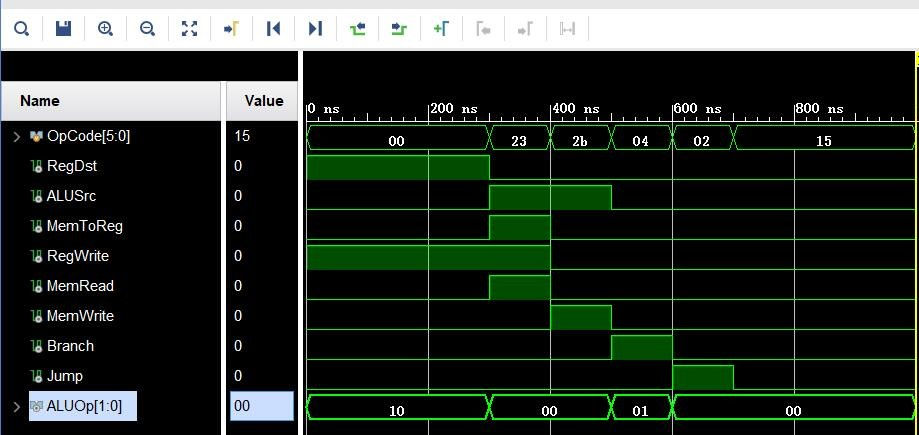
\includegraphics[width=0.9\textwidth]{fig-sim-ctr.jpg}
    \caption{主控制器模块的仿真结果}
    \label{fig:sim-ctr}
\end{figure}
仿真结果如图\ref{fig:sim-ctr}所示,我们实现的主控制器模块运行符合预期设计。

\subsection{算术逻辑单元控制器模块的仿真}
按照表\ref{tab:sim-aluctr}对算术逻辑单元控制器模块进行测试,仿真结果如图\ref{fig:sim-aluctr}所示。可见ALU控制器模块的输出结果符合预期。
\begin{table}[htbp]
    \centering
    \begin{tabular}{|c|c|c|}
    \hline
    ALUOp & Funct & 运算类型 \\
    \hline
    00 & xxxxxx & add \\
    01 & xxxxxx & sub \\
    10 & 100000 & add \\
    10 & 100010 & sub \\
    10 & 100100 & and \\
    10 & 100101 & or \\
    10 & 101010 & SLT \\
    \hline
    \end{tabular}
    \caption{仿真测试使用的ALUOp、Funct及解释}
    \label{tab:sim-aluctr}
    \end{table}

\begin{figure}[htbp]
    \centering
    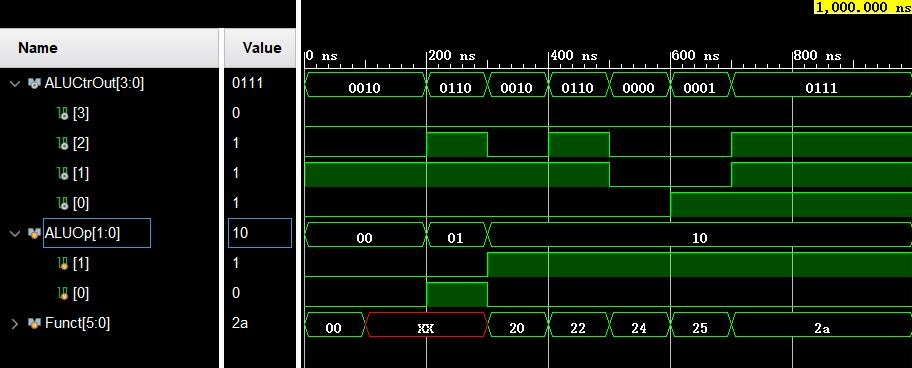
\includegraphics[width=0.9\textwidth]{fig-sim-aluctr.jpg}
    \caption{算术逻辑单元控制器模块的仿真结果}
    \label{fig:sim-aluctr}
\end{figure}

\subsection{ALU模块的仿真}
按照表\ref{tab:sim-alu}向ALU模块输入ALUCtr以及两个操作数,仿真结果如图\ref{fig:sim-alu}。ALU模块正确地完成了所有运算测试。
\begin{table}[htbp]
    \centering
    \begin{tabular}{|c|c|c|c|}
    \hline
    ALUCtr & 操作数1 & 操作数2 & 解释 \\ \hline
    0000 & 15 & 10 & 15 AND 10 \\
    0001 & 15 & 10 & 15 OR 10 \\
    0010 & 15 & 10 & 15 + 10 \\
    0110 & 15 & 10 & 15 - 10 \\
    0110 & 10 & 15 & 10 - 15 \\
    0111 & 15 & 10 & 15 < 10 \\
    0111 & 10 & 15 & 10 < 15 \\
    1100 & 1 & 1 & 1 NOR 1 \\
    1100 & 16 & 1 & 16 NOR 1 \\ \hline
    \end{tabular}
    \caption{ALU仿真使用的ALUCtr以及操作数}
    \label{tab:sim-alu}
    \end{table}

\begin{figure}[htbp]
    \centering
    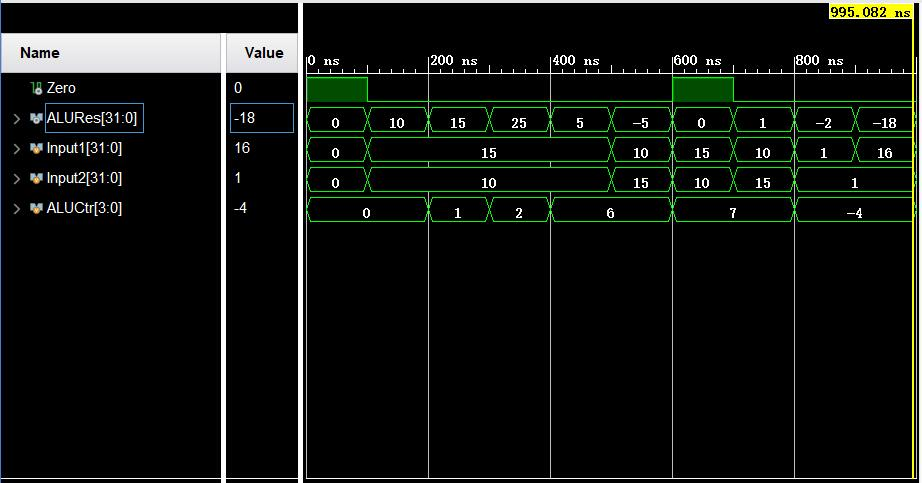
\includegraphics[width=\textwidth]{fig-sim-alu.jpg}
    \caption{ALU模块的仿真结果}
    \label{fig:sim-alu}
\end{figure}

\section{总结与反思}\label{sec4}
在本实验中,我实现了主控制器模块、ALU控制器模块、ALU模块。在开始实验之前,我本以为需要通过复杂的逻辑电路完成指令到控制信号的转换;开始试验后,我才知道可以通过Verilog的case与casex语句快速完成控制信号输出。实验难度比我的预期简单,这增加了我的信心。\par
在实验过程中,我曾经混淆了case与casex语句,在同学的帮助下,我顺利发现了错误并完成了实验。通过本实验,我对Verilog的分支语句、逻辑操作符有了初步了解。\par
本实验中实现的模块功能较为简单,主控制器模块只能识别少量指令,ALU控制器模块、ALU模块只能完成基础的加减法与逻辑运算,无法满足后续实验的需求;但是本实验完成了这些模块框架的搭建,后续实验可以便捷地根据需求拓展功能。作为处理器实现系列实验的开始,本实验难度适中,是一个非常合适的引入。

\end{document}